\subsection{Variação do comportamento da semelhança entre documentos}

Um dos meus objetivos foi analisar a variação do comportamento da semelhança entre os documentos de acordo com os valores dos parâmetros de 
treinamento. Conforme explicado anteriormente, a proximidade se dá pela da distância entre os documentos, que envolve um cálculo baseado
nas probabilidades que os documentos tem de terem em seu contexto identificados cada tópico. Quanto menor a distância entre os documentos, mais
próximos os mesmos e desta forma existe maior probabilidade de serem semelhantes.

Com base nisto eu resolvi analisar o comportamento da média e desvio padrão das distâncias de acordo com os parâmetros de treinamento ou outro fator
que pudesse influenciar na distância.

A tabela a seguir mostra que pelos resultados obtidos a média das distâncias entre documentos na fonte de origem utilizando o conjunto completo 
de páginas da Wikipedia foi menor que ao utilizar o conjunto de páginas limitado pelo tamanho. Isto mostra que mostra que o algoritmo considerou 
os documentos semelhantes mais próximos dos utilizados no treinamento para o conjunto completo.

\begin{center}
    \begin{tabular}{|c|c|c|}
        \hline
        Conjunto Wikipedia & Média de distâncias & Desvio padrão \\
        \hline
        full & 0.244593 & 0.169004 \\
        \hline
        gte40 & 0.293772 & 0.196154 \\
        \hline
    \end{tabular}
\end{center}

O histograma a seguir nos dá a mesma informação anterior, mas de forma gráfica. Podemos ver que para o conjunto completo há uma concentração
maior nas menores distâncias enquanto que o conjunto limitado tem maior concentração nas distâncias maiores.

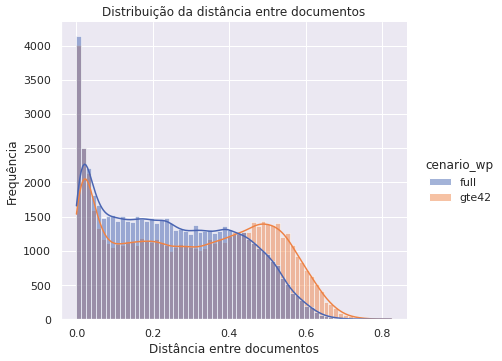
\includegraphics[scale=0.7]{resultados/resources/distribuicao_distancias.png}

O parâmetro \textbf{alpha} indica o comportamento da quantidade de tópicos que influenciam um conjunto de textos. Um valor baixo significa 
que os documentos tem um pequeno número de tópicos entre eles, ao passo que um valor alto indica que os documentos tem um maior número
de tópicos entre eles, ou seja, os documentos têm uma tendência a serem mais distintos em relação a outros.

Pelos valores abaixo percebemos que ao aumentar o valor de \textit{alpha} diminuem o valor das distâncias, ou seja, quanto dizemos ao algoritmo
que há mais tópicos dentro do conjunto de textos de treinamento, a tendência é que o algoritmo entenda que a proximidade com os documentos mais parecidos
da fonte de comparação seja maior.

\begin{center}
    \begin{tabular}{|c|c|c|}
        \hline
        Alpha & Média de distâncias & Desvio padrão \\ 
        \hline
        0.01 & 0.299975 & 0.202525 \\ 
        \hline
        0.10 & 0.327551 & 0.181500 \\ 
        \hline
        1.00 & 0.180020 & 0.126922 \\ 
        \hline
    \end{tabular}
\end{center}

O mesmo comportamento acima pode ser verificado graficamente. Com o valor de \textit{alpha} igual a 1, por exemplo, há uma concentração 
muito maior na área de distâncias menores.

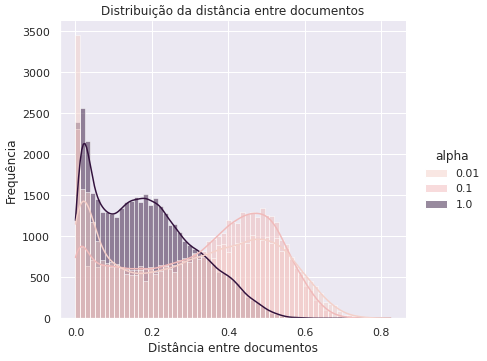
\includegraphics[scale=0.7]{resultados/resources/distribuicao_distancias_alpha.png}

O parâmetro \textbf{eta} indica o comportamento da quantidade de palavras que influenciam na definição dos tópicos. Um valor baixo significa 
que poucas palavras influenciam a definição de tópicos e vice-versa.

Pelos valores abaixo percebemos que ao aumentar o valor de \textit{eta} diminuem o valor das distâncias, ou seja, quanto dizemos ao algoritmo
que há mais palavras atuando na definição de tópicos dentro do conjunto de textos de treinamento, a tendência é que o algoritmo entenda que a 
proximidade com os documentos mais parecidos da fonte de comparação seja maior.

\begin{center}
    \begin{tabular}{|c|c|c|}
        \hline
        Eta & Média de distâncias & Desvio padrão \\ 
        \hline
        0.005 & 0.379512 & 0.150678 \\ 
        \hline
        0.050 & 0.371781 & 0.150373 \\ 
        \hline
        0.500 & 0.205030 & 0.152114 \\ 
        \hline
        1.000 & 0.120406 & 0.138177 \\ 
        \hline
    \end{tabular}
\end{center}

O mesmo comportamento acima pode ser verificado graficamente. Com o valor de \textit{eta} igual a 1, por exemplo, há uma concentração muito maior 
na área de distâncias menores.

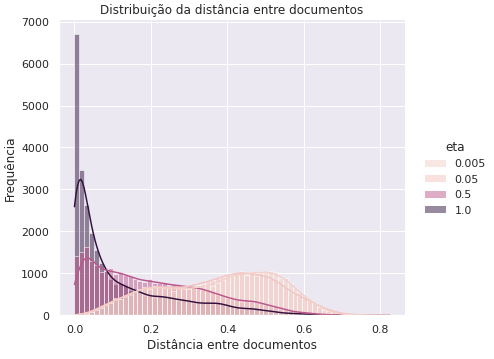
\includegraphics[scale=0.7]{resultados/resources/distribuicao_distancias_eta.png}

O número de tópicos a serem encontrados é outro parâmetro muito importante. Foi explicado anterior como o cálculo de coerência foi usado para definir 
a lista de números de tópicos que usamos em nossos testes. Abaixo segue uma tabela com o comportamento da variação das distância de acordo
com o número de tópicos. Percebemos que com menos tópicos este indicador de semelhança aumenta, já que na média temos distâncias menores.

\begin{center}
    \begin{tabular}{|c|c|c|}
        \hline
        Número de tópicos & Média de distâncias & Desvio padrão \\ 
        \hline
        22 & 0.234775 & 0.161470 \\ 
        \hline
        39 & 0.266610 & 0.173423 \\ 
        \hline
        45 & 0.270563 & 0.178036 \\ 
        \hline
        57 & 0.276523 & 0.184559 \\ 
        \hline
        67 & 0.285299 & 0.187543 \\ 
        \hline
        72 & 0.279334 & 0.191407 \\ 
        \hline
        101 & 0.271173 & 0.208681 \\      
        \hline
    \end{tabular}
\end{center}

O parâmetro \textbf{passes} indica o número de vezes que o algoritmo passa pelo conjunto de textos ao fazer o treinamento. Os valores abaixo indicam
que a diferença entre os dois valores utilizados (2 e 10) foi muito pequena, causando pouca influência na noção de proximidade entre os documentos.

\begin{center}
    \begin{tabular}{|c|c|c|}
        \hline
        Número de tópicos & Média de distâncias & Desvio padrão \\ 
        \hline
        2 & 0.265562 & 0.186465 \\ 
        \hline
        10 & 0.272802 & 0.182900 \\         
        \hline
    \end{tabular}
\end{center}

O mesmo comportamento anterior pode ser verificado na distribuição abaixo.

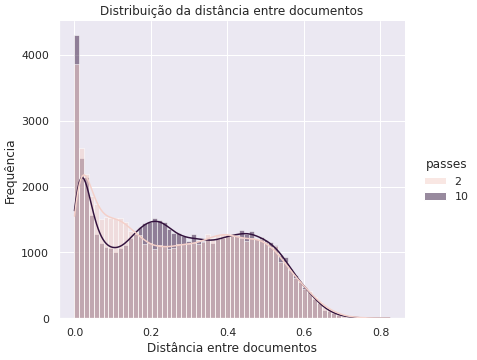
\includegraphics[scale=0.7]{resultados/resources/distribuicao_distancias_passes.png}
